%%
% 引言
% 引言是论文正文的开端,应包括毕业论文选题的背景、目的和意义;对国内外研究现状和相关领域中已有的研究成果的简要评述;介绍本项研究工作研究设想、研究方法或实验设计、理论依据或实验基础;涉及范围和预期结果等。要求言简意赅,注意不要与摘要雷同或成为摘要的注解。
%%

\chapter{引言}
\label{cha:introduction}

\section{问题背景}
\label{sec:background}
% What is the problem
% why is it interesting and important
% Why is it hards, why do naive approaches fails
% why hasn't it been solved before
% what are the key components of my approach and results, also include any specific limitations,do not repeat the abstract
%contribution

强化学习(Reinforcement Learning, RL)\cite{suttonReinforcementLearningIntroduction2018} \cite{ReinforcementLearning2021} \cite{salvadorREINFORCEMENTLEARNINGLITERATURE2020} 是机器学习(Machine Learning,  ML)领域的一部分。不同于监督学习,强化学习不需要带标签的学习样本, 而是利用奖励或惩罚智能体行为的方式间接设定学习目标。 RL 的灵感 \cite{ReinforcementLearning2021} 来源于心理学中的行为主义理论,即有机体如何在环境给予的奖励或惩罚的刺激下,逐步形成对刺激的预期,产生能获得最大利益的习惯性行为。理论上,强化学习可以达到人工智能(Artificial General Intelligence, AGI)\cite{salvadorREINFORCEMENTLEARNINGLITERATURE2020}。

在标准的强化学习 \cite{mnihAsynchronousMethodsDeep2016} 中,有几个重要的概念:智能体(agent),环境(environment),状态(state),动作(action)和奖励(reward)。考虑扫地机器人的场景:机器人通过在房间里移动和执行清扫动作,从而完成任务。如果有多个扫地机器人,如何挑选出“最好”的一个呢?我们可以计算每块地砖的清洁程度,设定合理的评分机制,从而挑选出得分最高的扫地机器人出来。如果从强化学习的角度看待这个问题,扫地机器人是智能体,房间里面的所有事物就是智能体所在的环境,智能体所在位置以及房间的形状、清洁程度就是改环境的状态,移动和执行清理动作是动作,而每块砖的清洁程度的增加量就是奖励,只是我们要训练出一个得分高的扫地机器人,而不是挑选出一个。现实中有很多这样的问题场景,例如棋盘游戏、电子游戏和自动驾驶等。我们抽象出强化学习的理论框架\cite{suttonReinforcementLearningIntroduction2018}:智能体是完成任务的机器,它负责学习和决策,而智能体执行任务过程中应对的外部事物是环境。这些事务之间持续进行交互,智能体选择动作,环境对这些动作做出响应,呈现出新的状态。同时智能体获取一个奖励,智能体的目标是最大化总的奖励。图 \ref{fig:agent-env-interaction} 展示了整个交互的过程,这将在第二章继续讨论。


\begin{figure}[h]
	\centering
	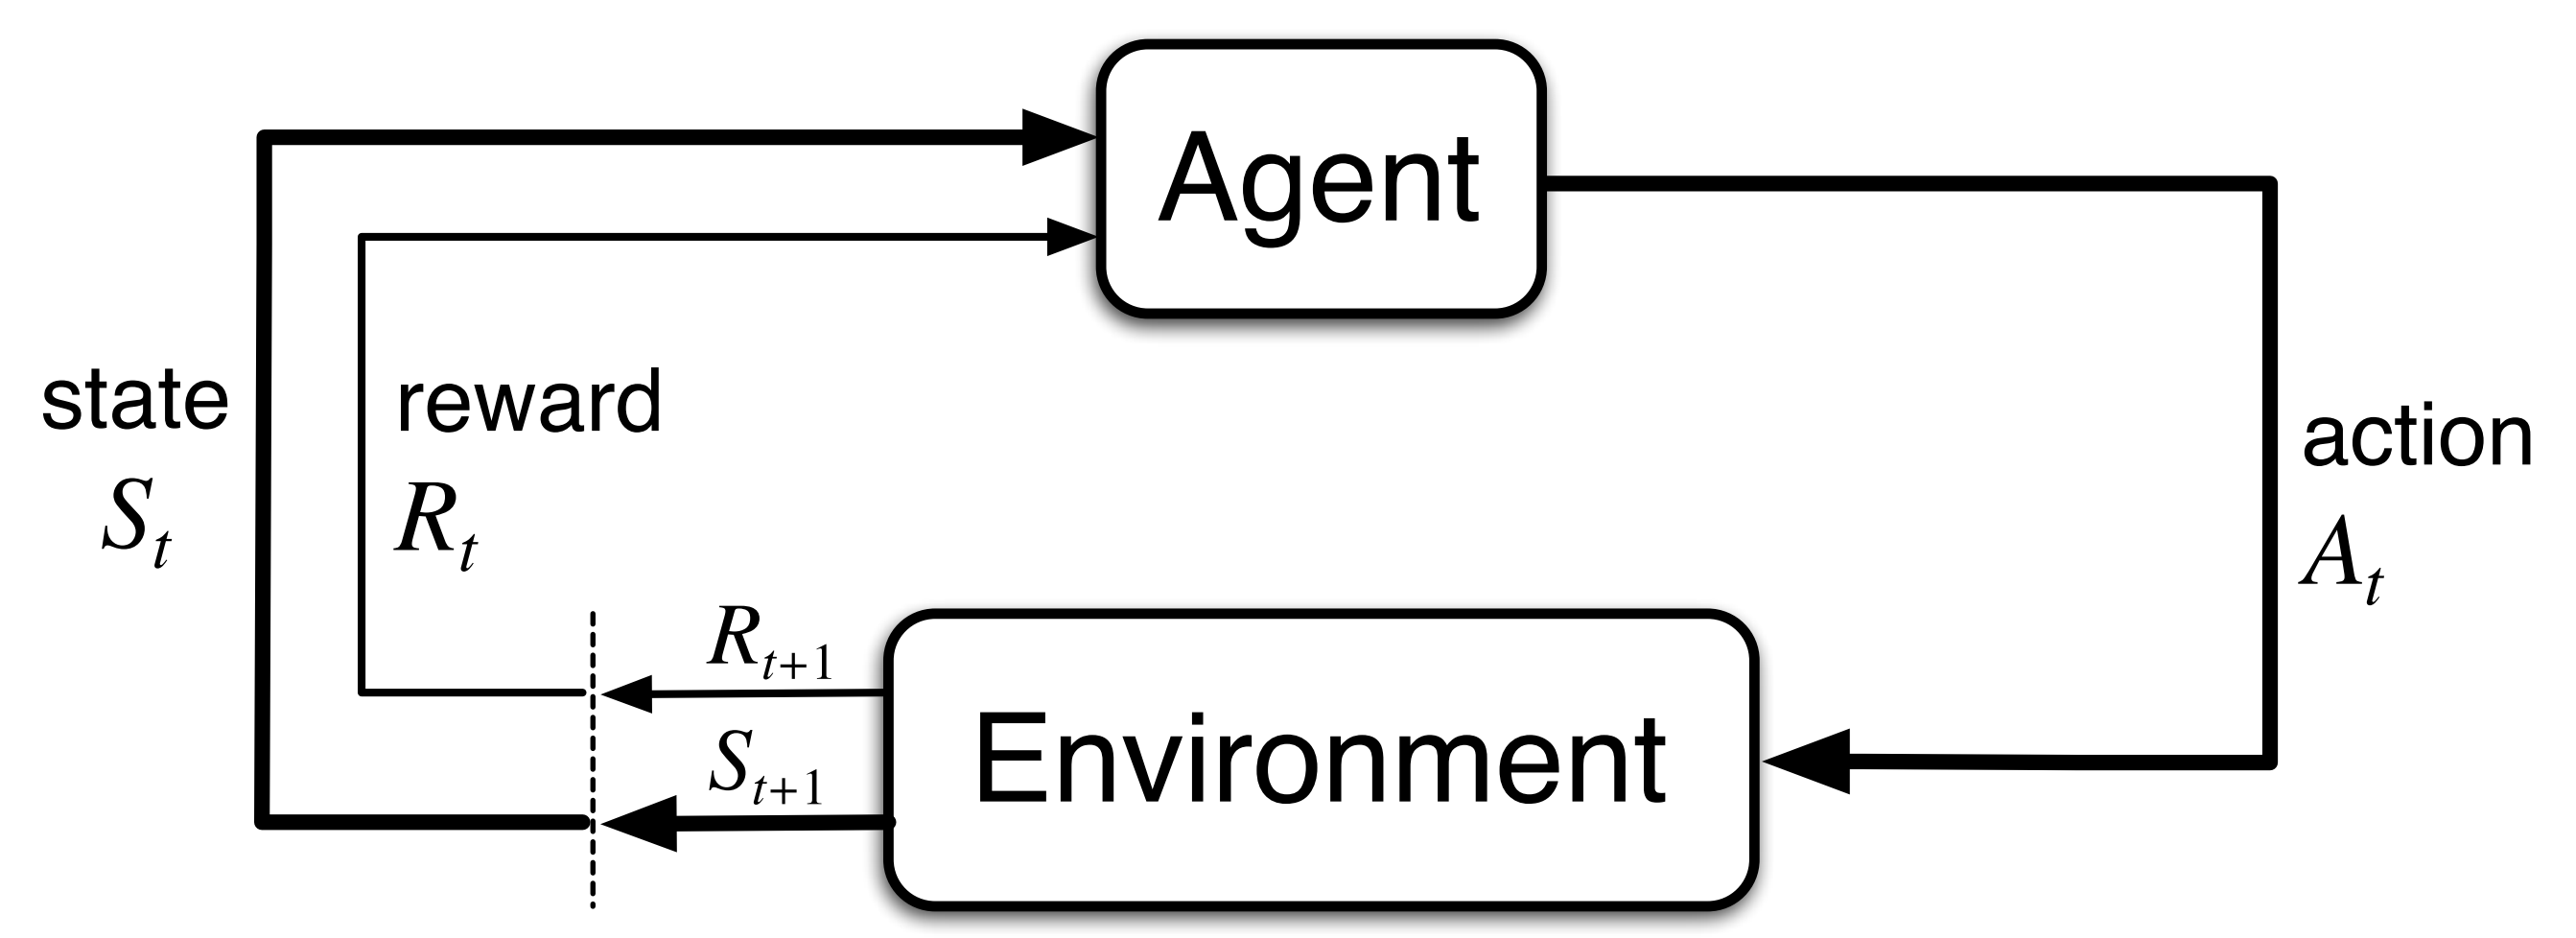
\includegraphics[width=0.9\textwidth]{image/chap01/interaction.png}
	\caption{智能体与环境交互过程\cite{suttonReinforcementLearningIntroduction2018}}
 	\label{fig:agent-env-interaction}
\end{figure}

% \section{强化学习介绍}
在上个世纪,对强化学习的研究已经有很多重要的理论和实践的成果出现\cite{suttonReinforcementLearningIntroduction2018}。过去的强化学习算法主要分为两类,以Q学习\cite{watkinsQlearning1992}算法为代表的基于值函数的方法和以策略梯度\cite{mnihAsynchronousMethodsDeep2016}算法为代表的基于策略的方法。
近些年来,由于深度学习技术的兴起,强化学习的研究和应用上取得巨大的成就。Mnih 等人提出了DQN 算法\cite{mnihPlayingAtariDeep2013} \cite{mnihHumanlevelControlDeep2015},该算法结合深度学习技术与经典的Q学习算法 \cite{watkinsQlearning1992},使得智能体在 Atari 游戏环境中的控制效果能达到人类的水平。当然,RL中最令人兴奋的成功案例之一是DeepMind公司开发的AlphaGo \cite{silverMasteringGameGo2016} 和AlphaZero \cite{silverMasteringGameGo2017} 围棋程序。AlphaZero可以玩国际象棋,围棋和其他游戏,相对于仅玩围棋的AlphaGo,它在性能和通用性方面都有改进。这些程序在其他几个方面也很出色。特别是,他们学会了如何在没有人工指导的情况下学会玩游戏。

大部分最近的强化学习相关工作并没有完全脱离原来的研究成果,而是以过去的研究所得的结论为理论基础的 \cite{ohDiscoveringReinforcementLearning2020}。然而,强化学习实践上许多棘手的问题例如稀疏奖励、不完全的状态观察、学习样本不够等等,在根据理想假设的理论上设计的基于值函数或者基于策略的方法并不能很好地解决。本文在这些算法的基础上,利用训练数据驱动学习的方式,探索更加适合问题的强化学习的策略更新算法,事实证明,这种方法是有一定效果的。

\section{相关工作}
\label{sec:related-work}

\subsection{比较早期的工作}
学习如何去学习(learning to learn),有时候也称为元学习(meta learning)\cite{MetaLearningComputer2021} 在早期工作里已经有各式各样的讨论。例如改进遗传程序设计\cite{ohDiscoveringReinforcementLearning2020} \cite{schmidhuberEvolutionaryPrinciplesSelfreferential1987},学习神经网络更新规则 \cite{bengioLearningSynapticLearning1990},学习率适应 \cite{suttonAdaptingBiasGradient1992} 和领域不变知识的转移\cite{thrunLearningOneMore1994}等等。此类工作表明,不仅可以学习优化固定目标,而且可以改进在元级别进行优化的方式,从而解决人为设计的学习规则不是完全适应问题本身的难题。


% 介绍普适性的元学习方法
\subsection{针对小样本的元学习}
对于小样本情形的机器学习,需要更高层次地设计,早期的一些工作从各个方面进行了研究。
Vinyals等人\cite{vinyalsMatchingNetworksOne2016b}(2016年)设计了可以学习一个网络结构的框架,有效地提升了图像分类任务的少样本学习的准确率。
Santoro 等人\cite{santoroMetaLearningMemoryAugmentedNeural2016}(2016年)设计了可以将过去的学习信息存储的增强记忆神经网络,该网络可以快速吸收新的数据,并利用此数据仅需几个样本就可以做出准确的预测。
Finn等人提出的 MAML(2017年)\cite{finnModelagnosticMetalearningFast2017} 和后来提出更通用的版本 \cite{finnMetaLearningUniversalityDeep2018}(2018年),通过先验的优化求解过程寻找更加适合求解优化问题的初始参数。
2017年 Duan 等人提出的 RL$^2$ 算法 \cite{duanRLFastReinforcement2016} 针对学习过程中实验次数过多问题,通过在代理的整个生命周期中展开LSTM,将学习本身描述为RL问题,从而利用过去的学习经验,减少在当前环境的训练次数。
所有这些方法都没有明确区分智能体和算法,所以,这些元学习算法也适用于单个智能体的程序结构。

% 单一环境任务下的元学习
\subsection{针对单一任务的元学习}
Xu等人\cite{xuMetagradientReinforcementLearning2018} (2018年)引入了元梯度RL方法。它使用反向传播遍历智能体程序的更新,以计算相对于更新的元参数的梯度。
该方法已应用于元学习各种形式的算法组件,例如折扣因子,内在奖励,辅助任务,回报以及辅助策略更新等\cite{ohDiscoveringReinforcementLearning2020}。然而,本文的工作与该方法的侧重点不一样,类似于LPG \cite{ohDiscoveringReinforcementLearning2020}:发现对更广泛的智能体和环境类别有效的通用算法,而不是适应特定的环境。

\subsection{元强化学习算法}
Houthooft 等人 在EPG \cite{houthooftEvolvedPolicyGradients2018} (2018年)使用进化策略来找到策略更新规则。
郑等人 \cite{zhengWhatCanLearned2020}(2018年)提出将奖励函数本身作为强化学习算法的表示的元学习框架,表明勘探的一般知识可以通过奖励函数的形式获得。
但是,先前的工作最多只能将相同领域中的相似任务概括化。
最近,Xu等人提出了 MetaGenRL \cite{kirschImprovingGeneralizationMeta2019} (2019年)来元学习领域不变的策略更新规则,该规则能够从几个 MuJoCo 环境推广到其他MuJoCo环境。
然而很少有先前的工作试图发现完整的更新规则;取而代之的是,它们全都依赖于价值函数(可以说是RL的最基本构建块)进行引导。
DeepMind公司在2020年提出的LPG元学习自举机制\cite{ohDiscoveringReinforcementLearning2020},该论文尝试使用LSTM模型学习到一个强化学习算法,而不是使用手工的方式定义一个梯度策略更新规则。该方法在特定的环境下表现比经典的优势动作者-评论者(advantage actor-critick,A2C)算法 \cite{mnihAsynchronousMethodsDeep2016} 的表现要好。然而该算法过于激进,完全不考虑人类知识对算法的改进。类似于此方法,不同的是,本文的方法将利用 A2C算法 进行启发式地探索新的强化学习算法;从另一个角度来看,本文的方法是寻找基于A2C算法的自适应策略更新算法。



\section{本文的论文结构与章节安排}
\label{sec:arrangement}

本文共分为五章,各章节内容安排如下:第一章提出文章的问题背景,同时介绍强化学习的作用和相关进展,然后介绍与本文相似的相关工作。 第二章是背景知识,介绍理解强化学习各个算法所必需的知识点。第三章是本文算法的详细描述,同时穿插着作者的考量。第四章是本文所提出的方法的实验验证,将本文方法与经典的算法进行对比,然后分析实验结果。第五章总结本文所有的工作,指出本文方法的优点和不足之处,并提出可能做的改进。
